
%(BEGIN_QUESTION)
% Copyright 2008, Tony R. Kuphaldt, released under the Creative Commons Attribution License (v 1.0)
% This means you may do almost anything with this work of mine, so long as you give me proper credit

Identify these different valve types from their respective diagrams:

\vskip 10pt

\noindent
{\bf Valve \#1:}

$$\includegraphics[width=15.5cm]{i00770x01.eps}$$

\vskip 10pt

\noindent
{\bf Valve \#2:}

$$\includegraphics[width=15.5cm]{i00770x02.eps}$$

\vskip 10pt

\filbreak
\noindent
{\bf Valve \#3:}

$$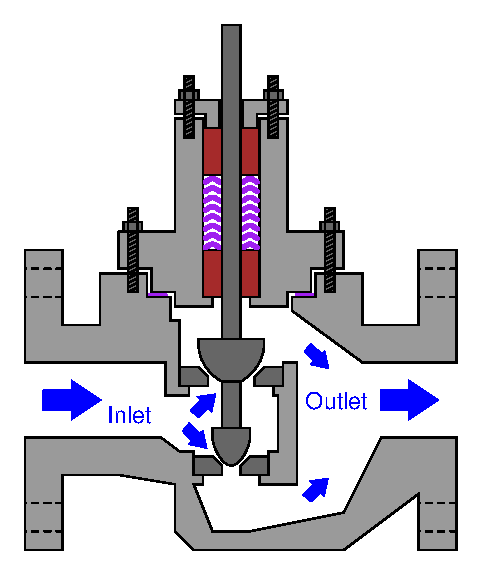
\includegraphics[width=15.5cm]{i00770x03.eps}$$

\vskip 10pt

\noindent
{\bf Valve \#4:}

$$\includegraphics[width=15.5cm]{i00770x04.eps}$$

\vskip 10pt

\filbreak
\noindent
{\bf Valve \#5:}

$$\includegraphics[width=15.5cm]{i00770x05.eps}$$

\noindent
{\bf Valve \#6:}

$$\includegraphics[width=15.5cm]{i00770x06.eps}$$



\underbar{file i00770}
%(END_QUESTION)





%(BEGIN_ANSWER)

Valve \#1: Ball valve (rotary)

\vskip 10pt

Valve \#2: Single-ported globe valve (sliding stem)

\vskip 10pt

Valve \#3: Dual-ported globe valve (sliding stem)

\vskip 10pt

Valve \#4: Saunders valve (diaphragm)

\vskip 10pt

Valve \#5: Gate valve (sliding stem)

\vskip 10pt

Valve \#6: Butterfly valve (rotary)

%(END_ANSWER)





%(BEGIN_NOTES)

%INDEX% Final Control Elements, valve: valve trim types

%(END_NOTES)


